\chapter{Marco Te\'orico}\label{chapter:state-of-the-art}

\section{Fundamentos de los Problemas de Satisfacci\'on de Restricciones y SAT}
\label{sec:fundamentos-sat-csp}

Los Problemas de Satisfacci\'on de Restricciones (CSP, por sus siglas en ingl\'es) constituyen un paradigma esencial para la modelaci\'on de problemas combinatorios en inteligencia artificial, investigaci\'on operativa y ciencias de la computaci\'on. Formalmente, un CSP se define como una tripleta $(V,D,C)$, donde $V$ representa un conjunto de variables, $D$ sus dominios discretos finitos, y $C$ un conjunto de restricciones que determinan las combinaciones v\'alidas de valores \cite{garcia_conferencia1}. Por ejemplo, en un problema de asignaci\'on de horarios, $V$ corresponde a los cursos, $D$ a los horarios disponibles, y $C$ a las reglas que impiden superposiciones. La soluci\'on del problema consiste en una asignaci\'on de valores a las variables que satisface todas las restricciones, y en algunos casos, adicionalmente, optimiza ciertos criterios como la utilizaci\'on de recursos \textbf{40}.

\subsection{SAT como Caso Especial de CSP y su NP-Completitud}
El Problema de Satisfacibilidad Booleana (SAT, por sus siglas en ingl\'es) se considera un caso particular de CSP, en el cual los dominios de las variables son binarios (${0,1}$) y las restricciones se expresan mediante f\'ormulas en Forma Normal Conjuntiva (FNC) \textbf{43}. Una f\'ormula en FNC se compone de una conjunci\'on de cl\'ausulas, donde cada cl\'ausula es una disyunci\'on de literales, es decir, variables o sus negaciones \textbf{6}. Resolver un problema SAT implica determinar si existe una asignaci\'on de valores que satisfaga simult\'aneamente todas las cl\'ausulas, lo cual equivale a resolver un CSP binario con restricciones espec\'ificas.

La importancia te\'orica de SAT se fundamenta en su clasificaci\'on como problema NP-completo, establecida por Cook y Levin en 1971 \textbf{2,24}. Esta clasificaci\'on conlleva dos implicaciones fundamentales: en primer lugar, cualquier problema perteneciente a la clase NP puede reducirse a una instancia de SAT en tiempo polinomial \textbf{26}; en segundo lugar, la existencia de un algoritmo de tiempo polinomial que resuelva SAT implicar\'ia que $P=NP$, lo cual provocar\'ia un colapso en la jerarqu\'ia de complejidad computacional \textbf{2}. Si bien en la pr\'actica los solucionadores actuales logran resolver instancias que contienen millones de variables \textbf{3}, en el peor de los casos SAT presenta una complejidad exponencial intr\'inseca \textbf{27}.

\subsection{Relación Práctica entre CSPs y SAT}
\label{subsec:csp-sat-relacion}

Si bien los CSPs permiten modelar problemas con dominios arbitrarios y restricciones globales —lo cual representa una ventaja frente a la rigidez booleana de SAT—, su resolución directa mediante técnicas como \textit{backtracking} o la aplicación de consistencia de arco presenta limitaciones similares en cuanto a escalabilidad \textbf{46}. Como respuesta a estas limitaciones, se recurre frecuentemente a la traducción de CSPs a SAT, con el objetivo de aprovechar las décadas de avances en la optimización de solucionadores CDCL\ref{subsection: cdcl} \textbf{44}. Estudios empíricos muestran que ciertas codificaciones eficientes pueden reducir hasta en un 60\% el tiempo de resolución en comparación con enfoques nativos basados en CSPs \textbf{45}.

Sin embargo, dicha traducción conlleva compromisos. Mientras SAT se adapta mejor a restricciones locales y cláusulas pequeñas, los CSPs ofrecen mecanismos más adecuados para el tratamiento de restricciones globales. En contextos como la asignación de turnos hospitalarios, los modelos CSP con restricciones de recursos logran resolver instancias en minutos, mientras que sus equivalentes codificados en SAT pueden requerir varias horas debido a la proliferación de cláusulas \textbf{46}. Esta dicotomía resalta la necesidad de seleccionar el paradigma de resolución en función de la estructura del problema.

%\begin{figure}[h]
%\centering
%\includegraphics[width=0.85\textwidth]{sat-csp-comparison.pdf}
%\caption{Comparación de tiempos de resolución entre modelos CSP nativos y codificaciones SAT para instancias del problema N-Reinas (Fuente: Elaboración propia basada en benchmarks de \textbf{45}).}
%\label{fig:sat-csp-comp}
%\end{figure}


\section{Evolución de los SAT \textit{solvers}: Principio de Resolución, DP, DPLL y CDCL}
\label{sec:evolucion-sat-solvers}
La evoluci\'on de los solucionadores SAT constituye un hito en la ciencia de la computaci\'on, pues convierte un problema te\'oricamente intratable en una herramienta pr\'actica de amplio uso industrial. Este desarrollo se apoya en tres pilares algor\'itmicos: el Principio de Resoluci\'on, los m\'etodos Davis-Putnam y Davis-Putnam-Logemann-Loveland, y la revoluci\'on moderna impulsada por los solucionadores de aprendizaje de cl\'ausulas dirigido por conflictos (\textit{Conflict Driven-Clause Learning}). A continuaci\'on, se presenta un an\'alisis detallado de cada uno.

\subsection{Principio de Resolución}
\label{subsec:prncp-de-res}
El Principio de Resolución (PR), propuesto originalmente en el contexto de la lógica proposicional, constituye la base teórica de numerosos algoritmos SAT. Este, permite derivar nuevas cláusulas a partir de pares de cláusulas que contienen literales complementarios, reduciendo progresivamente la fórmula hasta detectar una contradicción o verificar su satisfacibilidad. 

Dada una fórmula en Forma Normal Conjuntiva, cada una de sus cláusulas se representa como un conjunto de literales, y a su vez la f\'ormula se prepresenta como un conjunto de conjuntos. Por esta raz\'on no hay elementos repetidos dentro de una cláusula ni en la fórmula completa. Tomando como entrada esta representación, PR identifica pares de cláusulas que contienen literales complementarios ($q$ y $\neg q$) y genera una nueva cláusula al realizar la operaci\'n de uni\'on entre ellas y eliminando de cada una el literal y su opuesto. (citar libro de la L\'ogica Proposicional de Luciano)

Concretamente, si \(\mathbf{B}\) y \(\mathbf{C}\) son cláusulas de la FNC \(\mathbf{A}\) tales que \(l\in\mathbf{B}\) y \(\neg l\in\mathbf{C}\), entonces la cláusula resultante se define como:
\[
\mathbf{D}=(\mathbf{B}\setminus\{l\})\cup(\mathbf{C}\setminus\{\neg l\})
\]
En este proceso, \(\mathbf{B}\) y \(\mathbf{C}\) actúan como cláusulas padres o premisas, mientras que \(\mathbf{D}\) corresponde al solvente o conclusión.

Por ejemplo, la resolución de las cláusulas
\[
\{\neg p,\neg q,\neg r\}\quad y\quad\{\neg p,q,\neg r\}
\]
produce
\[
\{\neg p,\neg r\}
\]
Asimismo, la combinación de
\[
\{\neg q\}\quad y\quad\{q\}
\]
conduce a la cláusula vacía, lo que evidencia la insatisfacibilidad de la fórmula. (citar libro de la L\'ogica Proposicional de Luciano)

\subsubsection{Resoluci\'on Unitaria (RU)}
\label{subsubsec:res-unit}
Una instancia particular de PR es la Resoluci\'on Unitaria (RU), en la cual una de las premisas es una cl\'ausula unitaria\footnote{Una cl\'ausula que contiene un \'unico literal, y por tanto, fuerza su valor a ser verdadero bajo una interpretaci\'on determinada.}. Este caso especial adquiere relevancia por su simplicidad y eficiencia, ya que permite deducciones inmediatas a partir de asignaciones forzadas.

El proceso consiste en identificar una cl\'ausula unitaria y aplicar PR sobre otra cl\'ausula que contenga el literal complementario, elimin\'andolo y generando una nueva cl\'ausula m\'as restringida. Por ejemplo:

\begin{equation*}
\dfrac{\{\neg q, p, \neg r\},\{r\}}{\{\neg q, p\}}
\end{equation*}

En este caso, la cl\'{a}usula unitaria \( \{r\} \) permite simplificar la cl\'{a}usula \( \{\neg q, p, \neg r\} \), eliminando el literal \( \neg r \) y generando una nueva cl\'{a}usula \( \{\neg q, p\} \). Esta operaci\'{o}n puede aplicarse iterativamente, facilitando la propagaci\'{o}n de valores l\'{o}gicos en la f\'{o}rmula original, y constituye un componente fundamental en algoritmos como DPLL\ref{subsec:dpll} y CDCL\ref{subsection:cdcl}, donde se utiliza para propagar restricciones a lo largo del proceso de asignaci\'{o}n.

El Principio de Resoluci\'on, aunque es completo para fórmulas en FNC, su aplicación directa resulta impráctica debido al crecimiento exponencial en el número de cláusulas generadas \textbf{12}. Sin embargo, su relevancia conceptual fundamenta y guía el diseño de métodos más eficientes.


\subsection{Algoritmo Davis–Putnam (DP)}
\label{subsec:davis-putnam}
Uno de los primeros algoritmos propuestos para la resolución del problema SAT fue el de Davis-Putnam (DP), cuyo funcionamiento se basa en gran medida en el Principio de Resolución. Este algoritmo implementa tres procedimientos fundamentales: la Propagación Unitaria (PU), la Eliminación de Literales Puros (ELP) y la Resolución Basada en División (RD).

La Propagaci\'on Unitaria identifica cláusulas unitarias dentro de la FNC y procede a asignar forzosamente el valor correspondiente al literal involucrado. Seguidamente, elimina de la fórmula todas las cláusulas satisfechas por dicha asignación, y suprime el literal complementario en aquellas donde aparezca. Por su parte, la Eliminaci\'on de Literales Puros detecta literales cuya polaridad es única en toda la fórmula\footnote{se dice que $q$ es un literal puro en la FNC $A$ si $q$ ocurre en $A$ y $\neg q$ no} y elimina las cláusulas en las que aparezcan. Este procedimiento persigue la idea de que las cl\'ausulas con literales puros pueden satisfacerse directamente sin afectar la satisfacibilidad de la fórmula. Tanto PU como ELP se consideran técnicas de preprocesamiento destinadas a simplificar la FNC antes de aplicar los pasos recursivos del algoritmo.

Una vez realizadas estas simplificaciones, DP procede con la Resolución Basada en División, que consiste en seleccionar una variable, asignarle un valor (0 o 1) y continuar la resolución de forma recursiva a partir de la nueva fórmula. Esta estrategia permite explorar sistemáticamente el espacio de soluciones posibles hasta determinar si la fórmula es satisfacible o no. (citar libro de Luciano L\'ogica Proposicional)

V\'ease el siguiente ejemplo para una mejor comprensi\'on.

Sean las siguientes fórmulas de la Lógica Proposicional:

\begin{equation*}
    r, \quad [q \land r] \implies p, \quad [q \lor r] \implies \neg p, \quad [\neg q \land r] \implies \neg p, \quad \neg s \implies p
\end{equation*}

A partir de la conjunción de estas proposiciones, se obtiene la siguiente FNC:

\begin{equation*}
    \{\{r\}, \{p,\neg q, \neg r\}, \{\neg p, \neg q\}, \{\neg p, \neg r\}, \{\neg p, q, \neg r\}, \{p, s\}\}
\end{equation*}

Aplicando \textbf{Propagación Unitaria (PU)} sobre la cláusula unitaria $\{r\}$, se eliminan todas las cláusulas que contienen $r$ y se suprime $\neg r$ de las restantes:

\begin{equation*}
    \{\{p,\neg q\}, \{\neg p,\neg q\}, \{\neg p\}, \{\neg p,q\}, \{p,s\}\}
\end{equation*}

Posteriormente, al aplicar \textbf{PU} sobre la cláusula unitaria $\{\neg p\}$, se elimina toda cláusula que contenga $\neg p$ y se remueve $p$ de las demás:

\begin{equation*}
    \{\{\neg q\}, \{s\}\}
\end{equation*}

Aplicando nuevamente \textbf{PU} sobre $\{\neg q\}$:

\begin{equation*}
    \{\{s\}\}
\end{equation*}

Y finalmente, aplicando \textbf{PU} sobre $\{s\}$:

\begin{equation*}
    \{\}
\end{equation*}

Dado que la fórmula ha sido completamente reducida sin generar contradicciones, se concluye que la instancia es satisfacible. (citar libro de Luciano de L'ogica Proposicional)

Cabe señalar que el algoritmo Davis-Putnam requiere memoria exponencial en el peor de los casos, ya que explora todas las asignaciones posibles para las variables. Esto se traduce en un árbol de decisión cuyo tamaño crece exponencialmente con el número de variables involucradas.

\begin{figure}[ht]
    \centering
    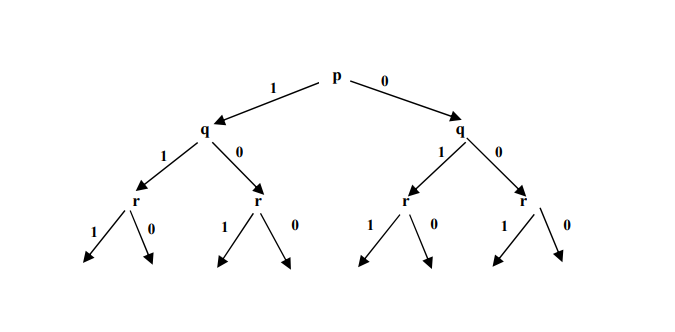
\includegraphics[width=0.8\textwidth]{Graphics/arboldp.png}
    \caption{Posible espacio de b\'usqueda de una FNC (citar libro de Luciano)}
    \label{fig:arbol DP}
\end{figure}


\subsection{Algoritmo Davis–Putnam–Logemann–Loveland (DPLL)}
\label{subsec:dpll}
El algoritmo Davis-Putnam-Logemann-Loveland (DPLL) constituye una mejora significativa del método DP, al preservar sus fundamentos teóricos y superar una de sus principales limitaciones: el consumo exponencial de memoria. Para ello, DPLL incorpora un mecanismo de retroceso (extit{backtracking}) cronológico que le permite deshacer asignaciones al regresar al nivel anterior de decisión una vez detectada una``cláusula de conflicto'' \footnote{Se denomina cláusula de conflicto a aquella en la que todos sus literales fueron evaluados como falsos bajo una asignación parcial.}. Este enfoque permite explorar el árbol de búsqueda de forma más eficiente, reduciendo la necesidad de almacenar todas las ramas posibles.

DPLL adopta una estrategia de generación ``lazy'' del árbol de asignaciones: antes de realizar una nueva ramificación, verifica mediante propagación unitaria si existen conflictos que invaliden dicha extensión. Esta verificación garantiza que las asignaciones parciales se mantengan consistentes, y que las soluciones (cuando existen) se ubiquen en las hojas del árbol de decisión. En caso de que el conflicto se produzca en el nivel de decisión cero, y ambas asignaciones posibles para la variable de este nivel hayan sido consideradas, se concluye que la fórmula es insatisfacible. En conjunto, el procedimiento de DPLL puede resumirse como una combinación de ramificación, propagación unitaria y retroceso sistemático.

Adicionalmente, DPLL incluye una etapa de preprocesamiento sobre la FNC, en la cual se aplican simplificaciones basadas en leyes de la L\'ogica Proposicional. Entre estas se encuentra la eliminaci\'on de cl\'ausulas redundantes mediante el principio de subsunci\'on\footnote{Sean $C$ y $C'$ dos cl\'ausulas de una FNC; si $C' \subseteq C$, entonces $C$ se considera subsumida por $C'$ y puede eliminarse sin alterar la satisfacibilidad de la f\'ormula. En otras palabras, $C$ es una cl\'ausula redundante.}. Estas t\'ecnicas contribuyen a reducir el tama\~no de la instancia antes de la b\'usqueda propiamente dicha, mejorando la eficiencia del algoritmo sin comprometer su completitud. (citar libro de Luciano)

Obsérvese el siguiente ejemplo:

Sea la FNC:

\begin{equation*}
\{\{\neg p,\neg q\},\{\neg p, \neg q\},\{\neg p,q,\neg r\},\{\neg p,r,s\},\{p,s\}\}
\end{equation*}

Simplificando mediante la ley de absorción:

\begin{equation*}
\{\{\neg p,\neg q\},\{\neg p,q,\neg r\},\{\neg p,r,s\},\{p,s\}\}
\end{equation*}

Eliminando el literal puro $s$:

\begin{equation*}
\{\{\neg p,\neg q\},\{\neg p,q,\neg r\}\}
\end{equation*}

Ramificando: $p = 1$

\begin{equation*}
\{\{\neg q\},\{q,\neg r\}\}
\end{equation*}

Aplicando \textbf{PU} en $\{\neg q\}$:

\begin{equation*}
\{\{\neg r\}\}
\end{equation*}

Aplicando \textbf{PU} en $\{\neg r\}$:

\begin{equation*}
\emptyset
\end{equation*}

Luego, la FNC es satisfacible. (citar libro de Luciano)

No obstante la reducción del espacio de memoria de DPLL respecto a DP, aún persisten problemas fundamentales: la selección de variables, el \textit{backtrack} cronológico y la elección de cláusulas unitarias.

En primer lugar, la selección de la variable a la que se asignará un valor influye directamente en la ``forma'' del espacio de búsqueda. Una decisión inapropiada puede derivar en caminos significativamente más largos hacia una solución. Por tanto, resulta crucial emplear heurísticas que optimicen esta elección. (poner ejemplo)

En segundo lugar, el \textit{backtrack} cronológico ante un conflicto obliga a explorar, posiblemente de forma innecesaria, las asignaciones alternativas en niveles anteriores. Esta ineficiencia se acentúa cuando la causa real del conflicto se encuentra a $k$ niveles de distancia del punto donde se detectó. Además, DPLL no capitaliza las cláusulas que originaron los conflictos; es decir, no ``aprende'' de ellos. En consecuencia, es susceptible de incurrir reiteradamente en los mismos patrones erróneos de asignación.

Finalmente, el problema de la selección de cláusulas unitarias también repercute en la eficiencia del algoritmo, estando íntimamente relacionado con la estrategia de selección de variables.



\subsection{\textit{Conflict-Driven-Clause-Learning} (CDCL)}
\label{subsection:cdcl}

CDCL es una mejora que se le a\~nadi\'o al algoritmo DPLL con el objetivo de erradicar el problema del retroceso (\textit{backtrack}) cronol\'ogico, una vez encontrada una cl\'ausula de conflicto.

El retroceso cronol\'ogico consiste en recorrer el \'arbol de decisi\'on (estructura propia del algoritmo DPLL que se forma al asignarle valores a las variables) retrocediendo de a 1 por cada nivel, probando todos los valores a\'un sin explorar de cada variable hasta encontrar la asignaci\'on causante del conflicto. Esta b\'usqueda es ineficiente pues adem\'as de analizar casos innecesarios, se vuelve susceptible a cometer el mismo error en el futuro dado que, potencialmente, realizar\'a la misma combinaci\'on de asignaciones, lo cual genera b\'usquedas redundantes.

Para solucionar este problema, CDCL crea un grafo dirigido y ac\'iclico que permite guardar el historial de asignaciones de cada variable. En dicho grafo, los nodos son las variables y los arcos constituyen la causa de la asignaci\'on de dicha variable: la cl\'ausula a la que pertenece, si fue asignada por propagaci\'on unitaria, y \texttt{null} para variables asignadas por decisi\'on. Igualmente, se almacenan los siguientes datos: el valor asignado a cada variable (0 o 1) y el nivel de decisi\'on en el que se asign\'o (los diferentes niveles de decisi\'on est\'an marcados por la asignaci\'on de valores por decisi\'on). Cabe destacar que la direcci\'on de los arcos en el grafo va desde las variables de decisi\'on hacia aquellas que, en el mismo nivel, tuvieron que forzar su valor por propagaci\'on unitaria. En el caso de una nueva variable de decisi\'on, se crea un nuevo arco con valor \texttt{null} desde la variable asignada por decisi\'on en el nivel anterior hasta la nueva variable. (insertar img de ejemplo de grafo)

Cuando una cl\'ausula resulta ser de conflicto (sus literales evaluaron 0), CDCL crea un nuevo nodo en el grafo que representa dicho conflicto para comenzar con su an\'alisis. Este, busca en el grafo la asignaci\'on causante del conflicto, para retroceder justo hacia ese punto y realizar un \textit{backjump} en lugar de un retroceso cronol\'ogico, como en DPLL. En caso de que el nivel del \textit{backjump} sea el nivel 0, CDCL considera la FNC como insatisfacible. Asimismo, con este an\'alisis CDCL busca conformar una ``cl\'ausula aprendida'' que represente la combinaci\'on de asignaci\'on de valores que condujo a dicho conflicto, y la a\~nade al conjunto de cl\'ausulas. De esta forma, evita cometer el mismo error en iteraciones futuras. El punto escogido para realizar el \textit{backjump} es conocido como primer punto de implicaci\'on \'unico (\textit{First-UIP} por sus siglas en ingl\'es). Este punto ser\'a aquel literal que, en la cl\'ausula aprendida, posea el m\'as alto nivel de decisi\'on diferente del actual. (annadir figura de First-UIP en el grafo)

Es necesario enfatizar en el hecho de que la cl\'ausula aprendida debe contener \textbf{\'unicamente} un literal cuyo valor haya sido asignado en el nivel de decisi\'on actual. En caso de haber m\'as de uno, CDCL recorre el grafo en busca de la cl\'ausula que caus\'o la asignaci\'on de una de estas variables y aplica el PR entre esta y la cl\'ausula aprendida hasta el momento. La cl\'ausula resultante pasar\'a a ser la nueva cl\'ausula aprendida. El proceso se repetir\'a hasta que la cl\'ausula aprendida contenga solo un literal cuyo valor fue asignado en el nivel de decisi\'on actual.

En el c\'odigo \href{Graphics/dpll\_cdcl\_sat\_solver.py}{Abrir c\'odigo fuente} se muestra un ejemplo de implementación en \textit{Python} de un CDCL SAT \textit{solver}

La implementación anterior consiste en una clase \textit{SATSolver} que realiza los pasos del algoritmo CDCL, dada una FNC escrita como un \textit{array} de \textit{arrays}, donde estos últimos representan las cláusulas. Cada variable está representada por un número entero positivo, y sus literales son ese número o su opuesto (negado).

El método \textit{\_\_init\_\_(self, formula)} inicializa las estructuras internas:
\begin{itemize}
  \item \textit{assignments}: Mapea cada variable con su valor asignado (\textit{True} o \textit{False}).
  \item \textit{levels}: Mapea cada variable con el nivel de decisión en que fue asignada.
  \item \textit{reasons}: Mapea cada variable con la cláusula que forzó su asignación, o \textit{None} si fue por decisión. Estos funcionan como los ``arcos'' del grafo de decisión.
  \item \textit{decision\_level}: Guarda el nivel actual de decisión.
  \item \textit{decision\_stack}: Pila que registra el historial de asignaciones como tuplas: (variable, valor, nivel de decisión).
\end{itemize}

El bucle principal del algoritmo se encuentra en el método \textit{solve(self)}. Mientras no se detecte un conflicto, asigna valores a variables no asignadas, actualizando las estructuras del solver. Si no quedan variables por asignar, devuelve la asignación completa y declara la fórmula como satisfacible. Si se detecta una cláusula conflicto y el nivel actual de decisión es 0, entonces devuelve \textit{None}, declarando que la fórmula es insatisfacible. 

El método \textit{unit\_propagate(self)} realiza propagación unitaria dentro de un ciclo de punto fijo que se repite mientras haya cambios (es decir, mientras existan cláusulas unitarias). Si se encuentra una cláusula conflicto, se detiene y la devuelve. Si no hay conflicto, retorna \textit{None}. Para determinar el estado de una cláusula (\textit{'satisfied'}, \textit{'conflict'}, \textit{'unit'}, \textit{'undefined'}), se utiliza el método \textit{check\_clause(self, clause)}.

Cuando se detecta una cláusula conflicto, se invoca \textit{conflict\_analysis(self, conflict\_clause)}. Este analiza cuántos literales de la cláusula conflicto fueron asignados en el nivel de decisión actual. La cláusula aprendida debe contener exactamente un literal asignado en ese nivel. Si hay más de uno, se identifica el último literal asignado (según el grafo de decisión), se busca la cláusula que causó su asignación y se aplica el Principio de Resolución entre ella y la cláusula aprendida. Este proceso se repite hasta obtener una cláusula con un solo literal en el nivel actual.

Luego, se determina el \textit{backjump level}, es decir, el nivel de decisión más alto presente en los literales de la cláusula aprendida (distinto del actual). Si este nivel es 0, CDCL considera la FNC como insatisfacible. Finalmente, se invoca el método \textit{backjump(self, level)} que deshace las asignaciones por encima del nivel objetivo y actualiza las estructuras correspondientes.

CDCL resuelve los problemas de b\'usquedas redundantes y \textit{bactrack} cronol\'ogico de DPLL, sin embargo, a\'un deja pendientes por resolver problemas como la selecci\'on de variables.


\section{Heur\'isticas}
\label{sec:heuristicas}

\subsection{\textit{Dynamic Largest Individual Sum} (DLIS)}
\label{sec}
La heur\'istica \textit{Dynamic Largest Individual Sum} es un m\'etodo aproximado de selecci\'on de variables que busca hacer eficiente la selecci\'on de variables en un CDCL SAT \textit{solver}. Para ello, DLIS considera que la pr\'oxima variable a asignar ser\'a aquella cuyo literal (el de mayor valor) tenga la mayor frecuencia de aparici\'on en cl\'ausulas insatisfechas. Es decir, para una variable $x$, se calcula la cantidad de cl\'ausulas no satisfechas en las que aparece el literal $x$ (forma positiva) y su complemento $\neg x$ (forma negativa). Denotemos:

\begin{itemize}
  \item $\textit{count\_pos}(x)$: cantidad de veces que $x$ aparece positivamente en cl\'ausulas insatisfechas.
  \item $\textit{count\_neg}(x)$: cantidad de veces que $\neg x$ aparece en cl\'ausulas insatisfechas.
  \item $\textit{dlis}(x) = \max(\textit{count\_pos}(x), \textit{count\_neg}(x))$.
\end{itemize}

La pr\'oxima variable a seleccionar ser\'a aquella que maximice el valor de $\textit{dlis}(x)$ entre todas las variables no asignadas:

\begin{equation*}
  x_k \mid \textit{dlis}(x_k) = \max(\textit{dlis}(x_i)),\quad i \in [1,n]
\end{equation*}

donde $n$ es el total de variables de la FNC.

Obs\'ervese que si $\textit{count\_pos}(x_k) > \textit{count\_neg}(x_k)$, entonces se asigna a $x_k$ el valor 1; en caso contrario, se asigna 0. El c\'alculo debe aplicarse solo a las variables no asignadas y solo considerar valores a\'{u}n no explorados en el nivel actual de decisi\'on.

Esta heur\'istica busca satisfacer la mayor cantidad de cl\'ausulas posibles en un mismo nivel de decisi\'on.

Tomando como base el algoritmo \href{Graphics/dpll\_cdcl\_sat\_solver.py}{Abrir c\'odigo fuente}, una forma de integrar DLIS ser\'ia como se muestra en \href{Graphics/dpll\_cdcl\_dlis\_sat\_solver.py}{Abrir c\'odigo fuente}. Esta estrategia de selecci\'on de variables puede integrarse en el algoritmo CDCL previamente presentado, sustituyendo la funci\'on \texttt{pick\_branching\_variable(self)} por una versi\'on que implemente la heur\'istica DLIS.

Las estructuras \texttt{pos\_counts} y \texttt{neg\_counts} se utilizan para almacenar, respectivamente, la cantidad de veces que el literal positivo y el literal negativo de cada variable no asignada aparece en las cláusulas actualmente insatisfechas. Este conteo es esencial para aplicar la heurística DLIS (\textit{Dynamic Largest Individual Sum}) de forma efectiva.

El procedimiento comienza recorriendo todas las cláusulas de la fórmula. Por cada cláusula que no esté satisfecha, se inspeccionan sus literales, y se incrementa el contador correspondiente de cada literal no asignado. Por ejemplo, si un literal positivo $x$ aparece en una cláusula insatisfecha, se incrementa \texttt{pos\_counts[$x$]}, y si aparece su complemento $\neg x$, se incrementa \texttt{neg\_counts[$x$]}.

Luego de este recorrido, se identifican todas las variables no asignadas que podrían no haber sido contadas, ya que podrían aparecer solamente en cláusulas ya satisfechas. A estas variables se les inicializa ambos contadores (positivo y negativo) en cero para garantizar una evaluación completa.

A continuación, se calcula el \textit{score} para cada variable no asignada, definido como el máximo entre \texttt{pos\_counts[$x$]} y \texttt{neg\_counts[$x$]}. Este valor representa la cantidad máxima de cláusulas que podrían satisfacerse al asignarle a la variable el valor correspondiente. Las variables se ordenan según su \textit{score} en orden descendente, y se elige aquella con el \textit{score} más alto como la próxima variable a asignar. En caso de empate, se utilizan criterios secundarios como la suma total de apariciones y el índice de la variable.

El valor que se asigna a la variable seleccionada depende de cuál de los dos conteos es mayor. Si \texttt{pos\_counts[$x$]} es mayor que \texttt{neg\_counts[$x$]}, entonces se asigna el valor \texttt{True} (es decir, $x$), de lo contrario se asigna \texttt{False} (es decir, $\neg x$).

DLIS tiene como objetivo maximizar el número de cláusulas satisfechas con cada asignación, lo que en teoría podría reducir la cantidad total de decisiones requeridas para encontrar una solución o para detectar una contradicción. Sin embargo, su aplicación resulta costosa para instancias de gran tamaño, debido a que implica una revisión completa de todas las cláusulas insatisfechas en cada nivel de decisión. Esto conduce a una complejidad computacional de $O(n)$ por nivel, donde $n$ es el número total de literales en la fórmula.


\subsection{\textit{Variable State Independent Decaying Sum} (VSIDS)}
\label{subsec:vsids}

La heurística de selecci\'on de variables que plantea \textit{Variable State Independent Decaying Sum} (VSIDS), prioriza asignar valores a aquellas variables que hayan estado involucrados en conflictos recientes. Para ello, VSIDS mantiene un \textit{score} por variable que se incrementa cada vez que esta aparece en cláusulas aprendidas a partir de conflictos. Además, para evitar que variables involucradas en conflictos antiguos tengan mayor prioridad que los relacionados con conflictos recientes, cada cierta cantidad \( T \) de conflictos se actualizan los \textit{scores} de todas las variables multiplicándolas por un factor de ``decaimiento'' \(\alpha\), con \(0 < \alpha < 1\) (usualmente \(\alpha = 0.95\)). 

Tomando como base el ejmplo de implementaci\'on de CDCL\href{Graphics/dpll\_cdcl\_sat\_solver.py}{Abrir c\'odigo fuente}, este ser\'ia el flujo de funcionamiento:

\begin{enumerate}
    \item Se ejecuta el algoritmo CDCL.
    \item Si ocurre un conflicto, se añade la cláusula aprendida \(\mathbf{C_{learn}}\). Luego, para cada literal \( l \) en \(\mathbf{C_{learn}}\), se actualiza su \textit{score} con \(score(l) = score(l) + \delta\), donde \(\delta\) es un incremento positivo.
    \item Si se alcanza el conflicto número \( T \), se actualiza el incremento con \( \delta = \delta \times \alpha \), con \(0 < \alpha < 1\).
    \item Si no ocurre un conflicto, se selecciona la variable \( v \) cuyo literal \( l_v \) cumple que su \textit{score} es máximo entre todos los literales \( l_i \), con \( i = 1, 2, \ldots, 2n \), siendo \( n \) la cantidad de variables. Si \( l_v \) es positivo, se asigna el valor 1 a \( v \), y 0 en caso contrario.
\end{enumerate}

El método\href{Graphics/dpll\_cdcl\_vsids\_sat\_solver.py}{Abrir c\'odigo fuente} selecciona, de entre las variables aún no asignadas, aquella con el mayor \textit{score} de acuerdo con la estrategia VSIDS. Para implementar este comportamiento, se añade a la clase \textit{SATSolver} una estructura llamada \textit{activity}, la cual asocia a cada variable un valor numérico que representa su actividad o relevancia. Esta estructura se inicializa al comienzo de la ejecución inspeccionando todas las variables presentes en las cláusulas de la fórmula, como se muestra en \texttt{Graphics/dpll\_cdcl\_vsids\_sat\_solver.py}.

Durante la ejecución del algoritmo CDCL, la estructura \textit{activity} se actualiza dentro del método \textit{solve(self)}. En particular, cada vez que se detecta un conflicto y se aprende una nueva cláusula, se incrementa la actividad de todas las variables que aparecen en dicha cláusula. Además, para priorizar los conflictos más recientes, se aplica un factor de decaimiento a todas las variables\href{Graphics/dpll\_cdcl\_vsids\_sat\_solver.py}{Abrir c\'odigo fuente}.

De este modo, la heurística VSIDS logra priorizar variables relevantes en conflictos recientes, mejorando la toma de decisiones del solucionador sin necesidad de reexaminar toda la fórmula.

Esta heur\'istica est\'a entre las m\'as usadas en los CDCL SAT \textit{solvers} modernos.

\subsection{Reinicio (\textit{restart})}
\label{subsec:restart}

Las estrategias de \textit{restart} tienen como objetivo evitar que el algoritmo de CDCL se estanque en regiones locales del espacio de búsqueda. Para ello, se permite reiniciar el árbol de decisiones, es decir, eliminar todas las asignaciones realizadas hasta el momento y comenzar nuevamente desde el nivel de decisión cero. Sin embargo, se conservan las cláusulas aprendidas durante el proceso, así como la información acumulada por las heurísticas de selección de variables (por ejemplo, las actividades de las variables en VSIDS o los conteos en DLIS). Estas estrategias buscan que, al conservar el conocimiento adquirido (cláusulas aprendidas), el solucionador pueda explorar regiones más prometedoras del espacio de soluciones sin tener que recorrer nuevamente caminos improductivos.

Existen diversos criterios para decidir cuándo realizar un reinicio:

\begin{enumerate}
    \item \textbf{Fijo}: se realiza un reinicio después de un número fijo $k$ de conflictos. Esta es una estrategia sencilla pero poco adaptativa.

    \item \textbf{Geométrico}: el número de conflictos entre reinicios crece de forma geométrica según la relación $r_0 = b$, $r_i = \alpha \cdot r_{i-1}$ con $\alpha > 1$. Esta estrategia permite reinicios más frecuentes al principio, reduciéndose con el tiempo. Un valor muy grande de $\alpha$ puede hacer que los reinicios sean demasiado esporádicos, mientras que un valor muy pequeño puede provocar una sobrecarga de reinicios.

    \item \textbf{Luby}: utiliza la secuencia de Luby $(1,1,2,1,1,2,4,1,1,2,\dots)$ para definir los intervalos entre reinicios, según la fórmula $r_i = b \cdot \text{Luby}(i)$, donde $b$ es un parámetro base que define el tamaño mínimo del intervalo. Esta estrategia tiene fundamentos teóricos que justifican su uso en entornos donde no se conoce a priori una buena política de reinicio.

    \item \textbf{Glucose-style (basada en LBD)}: esta estrategia se basa en el cómputo de la medida \textit{Literal Block Distance} (LBD) de las cláusulas aprendidas. Dada una cláusula $C_{learn}$, su LBD se define como el número de niveles de decisión distintos a los que pertenecen sus literales:
    \begin{equation*}
        \text{LBD}(C_{learn}) = |\{ \text{level}(l)\mid l \in C_{learn} \}|
    \end{equation*}
    La idea es que una cláusula con menor LBD involucra decisiones más cercanas entre sí, lo que la hace más relevante para guiar el proceso de resolución. 

    Para implementar esta estrategia, se mantienen dos promedios móviles de los LBD: uno para una ventana rápida de conflictos recientes (por ejemplo, los últimos 50 o 100) y otro para una ventana más larga (por ejemplo, los últimos 1000). Denotando estos promedios como $\mu_r$ (rápido) y $\mu_l$ (lento), se define un umbral $T > 1$. Si se cumple la condición:
    \begin{equation*}
        \frac{\mu_r}{\mu_l} > T
    \end{equation*}
    entonces se considera que el solucionador está atrapado en una región poco productiva y se procede con un reinicio.
\end{enumerate}

La incorporación de estrategias de reinicio, particularmente aquellas adaptativas como Luby o Glucose-style, ha demostrado ser fundamental para el éxito de solucionadores modernos de SAT, ya que permiten alternar entre exploración y explotación de manera eficiente en espacios de búsqueda complejos.

Ussando como base el código anterior\href{Graphics/dpll\_cdcl\_sat\_solver.py}{Abrir c\'odigo fuente} de CDCL, una posible implementación para, por ejemplo, la estrategia Luby ser\'ia\href{Graphics/dpll\_cdcl\_luby\_sa\_solver.py}{Abrir c\'odigo fuente}.

Como se puede ver en el c\'odigo, Luby se ha integrado al algoritmo CDCL modificando su estructura de control de conflictos. Para ello, se define una funci\'on \texttt{luby(u, k)} que genera el k-\'esimo valor de la secuencia de Luby multiplicado por una unidad base \texttt{u}, la cual determina el n\'umero de conflictos que deben ocurrir antes de realizar un reinicio.

Dentro de la clase principal del solucionador, se inicializan los siguientes parámetros:

\begin{itemize}
    \item \texttt{unit\_run}: intervalo base de conflictos entre reinicios.
    \item \texttt{luby\_idx}: índice actual dentro de la secuencia de Luby.
    \item \texttt{conflicts\_since\_restart}: contador de conflictos desde el último reinicio.
    \item \texttt{next\_restart}: umbral de conflictos para el siguiente reinicio, calculado como \texttt{luby(unit\_run, luby\_idx)}.
\end{itemize}

Durante la ejecución del método \texttt{solve()}, cada vez que se detecta un conflicto y se realiza el correspondiente análisis y retroceso (“\textit{backjump}”), se incrementa el contador de conflictos. Luego, se verifica si el número acumulado de conflictos ha alcanzado el umbral definido por la secuencia de Luby. En caso afirmativo, se ejecuta un reinicio que implica:

\begin{itemize}
    \item Vaciar las estructuras de asignaciones, niveles de decisión, razones de propagación y la pila de decisiones.
    \item Reiniciar el nivel de decisión a cero.
    \item Calcular el nuevo umbral de reinicio actualizando el índice de Luby y recalculando \texttt{next\_restart}.
    \item Reiniciar el contador de conflictos desde el reinicio.
\end{itemize}

Cabe destacar que durante el reinicio no se eliminan las cláusulas aprendidas, lo cual permite conservar información valiosa obtenida en decisiones anteriores. Esta estrategia favorece la salida de áreas del espacio de búsqueda poco prometedoras, maximizando la posibilidad de encontrar una solución en regiones más relevantes del espacio de soluciones.

A pesar de los avances, la separación teórica entre \textit{solvers} CDCL con y sin reinicios continúa siendo una pregunta abierta relevante, dado que muchos resultados dependen intrínsecamente de los reinicios. %Understanding and Enhancing CDCL-based SAT Solvers.pdf

\subsection{\textit{Two Watched Literals (TWL)}}
\label{subsec:twl}

Una de las estrategias m\'as empleadas en solucionadores modernos de SAT para optimizar la propagaci\'on unitaria es \textit{Two Watched Literals (TWL)}. Esta t\'ecnica tiene como objetivo evitar el recorrido exhaustivo de todas las cl\'ausulas en cada paso de propagaci\'on, mediante la vigilancia de dos literales por cl\'ausula, denominados $l_1$ y $l_2$.

Durante la ejecuci\'on del algoritmo, si ambos literales vigilados en una cl\'ausula no han sido evaluados, o al menos uno de ellos tiene valor verdadero, entonces no es necesario revisar dicha cl\'ausula, ya que no es unitaria ni entra en conflicto. En caso contrario, si uno de los literales es asignado a falso, se intenta buscar dentro de la cl\'ausula otro literal que no haya sido evaluado o que tenga valor verdadero, con el fin de reemplazar al literal que fue asignado a falso. Si no se encuentra un reemplazo v\'alido y el otro literal vigilado a\'un no tiene valor, entonces la cl\'ausula se vuelve unitaria, forzando la asignaci\'on del segundo literal. Si ambos literales vigilados son evaluados a falso, la cl\'ausula se considera en conflicto.

Esta estrategia resulta altamente eficiente, ya que disminuye considerablemente el n\'umero de cl\'ausulas que deben revisarse en cada nivel de decisi\'on, optimizando as\'i el rendimiento del algoritmo CDCL.

Para integrar la estrategia TWL en el c\'odigo base de CDCL, es necesario modificar la estructura interna del solucionador, incluyendo los m\'etodos de propagaci\'on, asignaci\'on y retroceso, entre otros. El c\'odigo de ejemplo es \href{Graphics/dpll\_cdcl\_twl\_sat\_solver.py}{Abrir c\'odigo fuente}.

La implementaci\'on del algoritmo CDCL puede enriquecerse significativamente mediante la integraci\'on del esquema Two Watched Literals (TWL), el cual transforma de manera sustancial la manera en que se gestiona la propagaci\'on unitaria.

En la versi\'on b\'asica de CDCL\href{Graphics/dpll\_cdcl\_sat\_solver.py}{Abrir c\'odigo fuente}, el procedimiento de propagaci\'on unitaria examina exhaustivamente todas las cl\'ausulas de la f\'ormula para identificar aquellas que se reducen a una sola literal no asignada bajo la interpretaci\'on parcial actual. En contraste, el enfoque basado en TWL introduce una estructura auxiliar que asigna a cada cl\'ausula exactamente dos literales que act\'uan como ``vigilantes''. Mientras al menos uno de ellos no est\'e asignado a falso, se garantiza que la cl\'ausula no puede causar conflicto ni ser unitaria, permitiendo as\'i omitir su revisi\'on durante la propagaci\'on.

El impacto de esta estrategia se observa en la estructura del c\'odigo. En la implementaci\'on enriquecida, se incorpora un diccionario que mapea cada literal a una lista de \'indices de cl\'ausulas que lo est\'an ``observando''. Esta organizaci\'on permite que, ante la asignaci\'on de un literal, solo se revisen aquellas cl\'ausulas que lo tienen como vigilante, reduciendo de forma dr\'astica la cantidad de cl\'ausulas analizadas en cada nivel de decisi\'on. Adem\'as, se redefine el procedimiento de propagaci\'on unitaria para que, al detectar que un literal vigilado ha sido evaluado a falso, se intente encontrar otro literal en la cl\'ausula que pueda ocupar su lugar como nuevo vigilante. Si esto no es posible y el otro literal vigilado tampoco satisface la cl\'ausula, se deduce que esta es unitaria o de conflicto, y se act\'ua en consecuencia.

Adem\'as de modificar la propagaci\'on unitaria, la estrategia TWL afecta tambi\'en la gesti\'on de cl\'ausulas aprendidas. Cada vez que se genera una nueva cl\'ausula como resultado del an\'alisis de conflictos, se seleccionan dos de sus literales para ser vigilados y se actualizan las estructuras de observaci\'on en consecuencia. Esto asegura que las optimizaciones ofrecidas por TWL se mantengan vigentes incluso cuando la f\'ormula evoluciona durante la ejecuci\'on del algoritmo.

La transici\'on desde un esquema de propagaci\'on unitaria tradicional hacia un enfoque basado en TWL representa una mejora sustancial en t\'erminos de eficiencia algor\'itmica. Al limitar el conjunto de cl\'ausulas a inspeccionar en cada paso, se logra una aceleraci\'on significativa del proceso de inferencia, lo cual resulta especialmente beneficioso en instancias de gran escala, donde los costos de propagaci\'on pueden dominar el tiempo total de ejecuci\'on.


\section{CaDiCaL}
\label{sec:cadical}

CaDiCaL es un \textit{solver} SAT moderno implementado en C++ que combina claridad de diseño y eficiencia práctica. La arquitectura se organiza en un módulo interno, responsable de la búsqueda CDCL y de técnicas de simplificación de fórmulas; y en un módulo externo que actúa como fachada, gestiona la API y, en modo incremental, revierte pasos de \textit{inprocessing} para mantener limpia la pila de reconstrucción.

\subsection{Ramificaci/'on (selecci\'on de variables)}
Las decisiones de ramificación se guían por heurísticas de actividad basadas en VSIDS, alternando entre fases estables y enfocadas para mejorar el rendimiento en instancias satisfacibles. %Combining VSIDS and CHB using restart in SAT.pdf  
%Unit Propagation with Stable Watches.pdf

\subsection{Políticas de reinicio}
\label{subsec:cadical-restart}

CaDiCaL implementa políticas de reinicio dinámicas que se ajustan al comportamiento interno del \textit{solver}. %Evaluating CDCL Restart Schemes.pdf, Revisiting Restarts of CDCL Should the Search Information be Preserved.pdf
Estos reinicios, permiten al solucionador escapar de subespacios improductivos sin perder las cláusulas aprendidas. Para ello, CaDiCaL emplea políticas adaptativas que utilizan contadores de eventos (por ejemplo, accesos a memoria) en lugar de mediciones temporales directas, lo que garantiza determinismo entre ejecuciones. Estas políticas bloquean reinicios cuando la búsqueda se encuentra próxima a una solución potencial, siguiendo estrategias propuestas en la literatura. %Combining VSIDS and CHB Using Restarts in SAT.pdf  
%Evaluating CDCL Restart Schemes.pdf  
%Revisiting Restarts of CDCL Should the Search Information be Preserved.pdf
Todas las \textit{restart policies} pueden ajustarse mediante múltiples parámetros para adaptarse a las características de cada instancia. %Better Decision Heuristics in CDCL through Local Search and Target Phases.pdf

CaDiCaL alterna entre dos modos operativos principales: modo estable y modo enfocado. En el modo estable, se utilizan reinicios tipo Luby\ref{subsec:restart} con un intervalo base elevado (1024 conflictos). Este modo promueve estabilidad, realiza retrocesos cronológicos y aplica la heurística VSIDS con bajo factor de incremento. Por otro lado, en el \textbf{modo enfocado}, se aplican reinicios como \textit{Glucose-style}\ref{subsec:restart} con intervalos cortos entre reinicios (2 conflictos).

\subsection{\textit{Assumptions}}
\label{subsec:cadical-assumptions}
% ¿Qué son las 'assumptions'?

Las \textit{assumptions} permiten invocar un SAT \textit{solver} con un conjunto de valores previamente asignados a ciertas variables. Esta funcionalidad resulta particularmente útil en contextos donde el \textit{solver} se utiliza de manera iterativa.

Por ejemplo, si se requiere agregar o eliminar una cláusula $c_i$ entre distintas invocaciones al \textit{solver}, esta puede incorporarse a la fórmula como $(c_i \lor s_i)$, donde $s_i$ es una variable de activación, selección o indicador. Al asignar $s_i = 1$, la cláusula $c_i$ se incluye efectivamente en la fórmula; en cambio, al establecer $s_i = 0$, dicha cláusula se omite.

Esta técnica fue introducida originalmente en el \textit{solver} MiniSat. %Chapter 4 Conflict-Driven Clause Learning SAT Solvers Marquwa-Silva Handbook of Satisfiability 2021.pdf

Además de su uso en la resolución incremental, las variables de activación también se aplican para representar cláusulas temporales. Por ejemplo, para incorporar una cláusula temporal $c$, se introduce una variable de activación $a$ y se añade $(c \lor a)$ a la fórmula, bajo la suposición de $\neg a$. Para eliminar $c$, basta con agregar la cláusula unitaria $(a)$.

En versiones recientes, CaDiCaL ha incorporado el uso de \textit{constraints}, que pueden simularse a través de \textit{activation literals} en versiones anteriores. % Documento cadical

El incremento en el número de variables de activación puede afectar negativamente el rendimiento del \textit{solver}. Tradicionalmente, este inconveniente se ha abordado mediante reinicios periódicos. %Deeply Optimizing the SAT Solver fir the IC3 Algorithm.pdf

% ¿Por qué se comprueban antes de la heurística de decisión de variables?

Las \textit{assumptions} se asignan y se propagan antes de que se inicie la búsqueda efectiva mediante la heurística de decisión de variables. Esta ordenación obedece a la arquitectura de los \textit{solvers} CDCL (\textit{Conflict-Driven Clause Learning}). %Chapter 4 Conflict-Driven Clause Learning SAT Solvers Marquwa-Silva Handbook of Satisfiability 2021.pdf

El algoritmo CDCL comienza con una fase de propagación unitaria. Si la PU detecta un conflicto en el nivel de decisión 0 (es decir, antes de que el \textit{solver} haya realizado alguna decisión propia), se concluye que la fórmula, junto con las \textit{assumptions} actuales, es insatisfacible. %AutoSAT Automatically Optimize SAT Solvers via Large Language Models.pdf
Esta verificación temprana resulta fundamental para la eficiencia del proceso, ya que permite detectar la insatisfacibilidad sin necesidad de explorar el espacio de búsqueda a través de decisiones de ramificación que, eventualmente, conducirían a un conflicto inevitable debido a los supuestos. %%Chapter 4 Conflict-Driven Clause Learning SAT Solvers Marquwa-Silva Handbook of Satisfiability 2021.pdf

Solo si la PU no detecta conflictos y no todas las variables están asignadas, el \textit{solver} procede a seleccionar una variable para ramificar, utilizando la heurística de decisión correspondiente. %AutoSAT Automatically Optimize SAT Solvers via Large Language Models.pdf

Las \textit{assumptions} constituyen un punto de partida para el \textit{solver}. Estas se procesan inicialmente mediante la propagación unitaria, lo que permite verificar que la configuración inicial, incluyendo los supuestos, no conduzca a un conflicto inmediato. Esta estrategia optimiza el procedimiento, al evitar búsquedas infructuosas en regiones del espacio que se sabe de antemano que son inconsistentes con los supuestos proporcionados.

\subsection{\textit{Phasing}}
\label{subsec:cadical-phasing}
La estrategia de \textit{phasing} constituye un componente fundamental en los SAT \textit{solvers} basados en CDCL, ya que desempeña un papel crucial en la guía del proceso de búsqueda de soluciones.

En el contexto de los \textit{solvers} CDCL, una vez seleccionada una variable para ramificación, se debe decidir qué valor de verdad (también denominado \textit{fase} o \textit{polaridad}) asignarle. Esta decisión influye significativamente en la eficiencia del \textit{solver}, particularmente en fórmulas satisfacibles.

La técnica de \textit{phase saving} (ahorro de fases) consiste en registrar el último valor asignado a una variable (ya sea mediante decisión o propagación unitaria) y reutilizar este valor cuando la variable sea seleccionada nuevamente como variable de decisión. Esta técnica, sencilla y de bajo costo computacional, ha demostrado mejorar el rendimiento de forma notable y se ha convertido en un estándar en la mayoría de los \textit{solvers} CDCL modernos. Se clasifica como una estrategia de intensificación, al mantener la búsqueda dentro de regiones previamente exploradas y potencialmente prometedoras. %Better Decision Heuristics in CDCL through Local Search and Target Phases.pdf

\textit{Rephasing} (refaseo) es una técnica de diversificación que complementa el ahorro de fases. Su propósito es reiniciar o ajustar la asignación parcial de las fases, permitiendo al \textit{solver} explorar nuevas regiones del espacio de búsqueda. Dado que la selección de fase no compromete la corrección ni la terminación del algoritmo CDCL, las fases guardadas pueden modificarse arbitrariamente.%Better Decision Heuristics in CDCL through Local Search and Target Phases.pdf

CaDiCaL incorpora mecanismos avanzados tanto de ahorro de fases como de \textit{rephasing}. %Cadical 2.0
Ha sido pionero en la implementación de refaseo periódico, en el que los valores de fase se reinician en intervalos predefinidos durante la ejecución. 



% tOOOda esta vaina de la Modularidad y Extensibilidad del codigo tiene referencia a Cadical 2.0
\subsection{Modularidad y Extensibilidad del Código de CaDiCaL}
La modularidad y la extensibilidad constituyen objetivos esenciales en el diseño de CaDiCaL. %citar Cadical2.0. 
Este \textit{solver} se ha convertido en plantilla para el ``\textit{hack track}'' de la competencia SAT desde 2021, evidenciando su facilidad de adaptación. Los mecanismos principales para modificar su comportamiento incluyen:
\begin{itemize}
  \item \textbf{API rica}: proporciona una interfaz en C++ (y limitada en C) que permite extender funcionalidades y personalizar la interacción con el solver.
  \item \textbf{Propagadores de usuario (ExternalPropagator)}: habilita la implementación de propagadores externos capaces de importar y exportar cláusulas aprendidas o sugerir decisiones al solver, otorgando control directo sobre la búsqueda.
  \item \textbf{Estructura del código fuente}: el código, organizado de forma clara y modular, facilita su uso como modelo para portar e integrar técnicas de última generación en otros \textit{solvers}.
\end{itemize}
Diversas investigaciones han extendido CaDiCaL para incorporar nuevas características, algunas de las cuales se han integrado en la versión oficial.

\subsection{Ventajas de CaDiCaL para Experimentación}
CaDiCaL resulta adecuado para estudios académicos sobre heurísticas y políticas de reinicio en SAT solving por las siguientes razones:
\begin{itemize}
  \item \textbf{Diseño limpio y modular}: la arquitectura está orientada a la comprensibilidad y facilidad de modificación, lo que simplifica la implementación de nuevas estrategias sin la complejidad de otros solvers avanzados.
  \item \textbf{Flexibilidad en heurísticas y reinicios}: aunque dispone de configuraciones predeterminadas, permite alternar entre modos estable y enfocado, y ajustar esquemas de rephasing para probar variaciones en políticas de reinicio %BetterDecisionHeuristics.
  \item \textbf{Rendimiento competitivo}: mantiene un desempeño de última generación, garantizando que los resultados experimentales sean representativos del estado del arte.
  \item \textbf{Adopción en la comunidad}: su uso extendido en investigación genera un entorno colaborativo y recursos para investigadores.
  \item \textbf{Documentación exhaustiva}: el código fuente cuenta con comentarios detallados, facilitando la comprensión y manipulación del solver por parte de nuevos usuarios.
\end{itemize}
% Exceptuando el que esta indicado en esta seccion, todas las referencias son a Cadical 2.0



\section{Parámetros de Evaluación para \textit{solvers} CDCL: Taxonomía de extit{Benchmarks}}
\label{sec:tipos-problemas}
\subsection{Categor\'ias}
\label{subsec:problem-categor}
La evaluación sistemática de solvers CDCL exige una taxonomía clara de instancias SAT que permita comparar heurísticas de actividad, estrategias de reinicio y métodos de propagación unitaria. Para este propósito, las instancias se clasifican según su origen y propiedades estructurales, de modo que cada categoría revele puntos fuertes y limitaciones algorítmicas 	extbf{15,17}.

En primer lugar, las instancias de aplicaci\'on proceden de problemas industriales, como la verificación de circuitos o la planificación logística. Estas fórmulas presentan estructuras modulares y \textit{backdoors} pequeños (subconjuntos de variables cuya asignación simplifica significativamente la búsqueda), lo que permite a heurísticas dinámicas como VSIDS explotar patrones locales mediante el registro de conflictos recientes  \textbf{20,21,23}.

Por otro lado, las instancias combinatorias dificultosas, diseñadas para desafiar la generalidad de los solvers (por ejemplo, codificaciones del principio del palomar), carecen de la estructura implícita de los casos reales y exhiben simetrías y dependencias globales que ponen a prueba la adaptabilidad de las heurísticas  \textbf{16,19}.

Además, las instancias aleatorias, generadas según modelos Random $k$-SAT, muestran una distribución uniforme de cláusulas sin sesgos estructurales. En estas condiciones, técnicas como el aprendizaje de cláusulas ofrecen beneficios limitados, lo que resulta clave para evaluar el rendimiento en entornos carentes de regularidades 	extbf{17,21}.

\subsection{Clasificación por Satisfacibilidad y Propiedades Estructurales}
La distinción entre instancias SAT e UNSAT determina la orientación de las estrategias de resolución. En las primeras, las heurísticas que exploran asignaciones prometedoras (como VSIDS con preservación de fase\textit{ (phase saving)}) potencian la localización rápida de soluciones. Por su parte, las instancias UNSAT requieren la generación de cláusulas aprendidas de alto impacto, con el fin de acotar el espacio de búsqueda y acelerar la refutación \textbf{41}.

Del mismo modo, las propiedades estructurales aportan criterios de evaluación adicionales. La modularidad de la fórmula y la existencia de \textit{backbones} (variables que mantienen el mismo valor en todas las soluciones) facilitan la identificación de subespacios críticos.

\subsection{Densidad y Transición de Fase}
La densidad de una instancia, definida como el cociente entre cláusulas y variables, condiciona su nivel de dificultad. En los modelos aleatorios de 3-SAT, la complejidad alcanza su punto máximo alrededor de 4.26 cláusulas por variable, conocido como umbral de transición de fase \textbf{25}. En esta zona, heurísticas estáticas como DLIS pierden eficacia ante la ausencia de patrones explotables \textbf{17}. En cambio, la combinación de VSIDS con políticas de reinicio basadas en LBD equilibra la exploración global y la explotación local, permitiendo al \textit{solver} superar con eficiencia estas regiones críticas \textbf{21}.

\subsection{Relevancia para la Evaluación de Heurísticas}
La selección de \textit{benchmarks} resulta crucial al contrastar técnicas como VSIDS y DLIS. Mientras DLIS, basada en conteos estáticos de aparición de literales, ofrece un rendimiento óptimo en instancias aleatorias alejadas del umbral de transición de fase \textbf{18}, VSIDS prevalece en aplicaciones reales gracias a su adaptación dinámica a patrones de conflicto \textbf{30}.

\section{Problemas}
\label{sec:problemas-ej}

\subsection{Random $k$-SAT}
\label{subsec:random-k-sat}
Los problemas Random $k$-SAT son un tipo de instancias generadas aleatoriamente que se utilizan ampliamente para evaluar y caracterizar el rendimiento de los algoritmos SAT. También se conocen como modelos de longitud fija de cláusula y constituyen un objeto de estudio prominente en la literatura. %SAT and Constraint Satisfaction.pdf

En un problema Random $k$-SAT, se define un número de variables $n$, un número de cláusulas $m$ y una longitud fija de cláusula $k$. Para generar cada cláusula, se seleccionan $k$ literales de forma independiente y uniforme al azar del conjunto de posibles literales, que incluye las variables proposicionales y sus negaciones. No se incluyen cláusulas que contengan múltiples copias del mismo literal. El proceso de generación continúa hasta que la fórmula contiene el número total especificado de cláusulas $m$. %SAT and Constraint Satisfaction.pdf

Una propiedad destacada del Random $k$-SAT es la presencia de un fenómeno de transición de fase. Este fenómeno se manifiesta como un cambio abrupto en la solubilidad al variar sistemáticamente el número de cláusulas $m$ para un número fijo de variables $n$. Cuando $m$ es pequeño, casi todas las fórmulas son poco restringidas y, por ende, satisfacibles. Al alcanzar un valor crítico $m_c$, la probabilidad de que una instancia sea satisfacible disminuye abruptamente hasta casi cero. Más allá de este punto, la mayoría de las instancias se encuentran sobre\-restringidas y son insatisfacibles. Para el caso de Random 3-SAT, esta transición ocurre aproximadamente cuando la razón cláusulas/variables ($m/n$) es cercana a 4.26 para valores grandes de $n$. La dificultad de los problemas SAT alcanza su punto máximo en esta región de transición. %On The Unreasonable Effectiveness of SAT Solvers.pdf, SAT and Constraint Satisfaction.pdf

\subsection{Problema del palomar}
\label{subsec:pingeonhole}
El ``problema del palomar'' (\textit{pigeonhole problem}) es una instancia de problema de Satisfacibilidad Booleana (SAT) que se ha convertido en un punto de referencia en la investigación de solvers SAT. A pesar de ser un problema combinatorio de tamaño relativamente pequeño, presenta dificultades particulares para los solvers CDCL (Conflict-Driven Clause Learning).

Este problema es un ejemplo de fórmulas “artesanales” o generadas aleatoriamente que resultan difíciles para los solvers CDCL. %Understanding and Enhancing CDCL-based SAT Solvers.pdf
Se considera una de las clases de problemas para los cuales los solvers CDCL son ``sin esperanza'' en la demostración de insatisfacibilidad, dado que cualquier prueba de refutación por resolución requerirá un tamaño exponencial. %Improving SAT Solvers by Exploiting Empirical Characteristics of CDCL.pdf

Este comportamiento contrasta con la eficiencia que muestran los solvers CDCL para problemas industriales o del mundo real. %Understanding and Enhancing CDCL-based SAT Solvers.pdf
La dificultad radica en que los solvers CDCL no pueden generar pruebas de refutación sofisticadas de manera eficiente para este tipo de instancias, a diferencia de los problemas industriales donde sí pueden hacerlo. %Improving SAT Solvers by Exploiting Empirical Characteristics of CDCL.pdf

El problema del palomar se usa como ejemplo para entender por qué los solvers CDCL son eficientes en muchas clases de instancias del mundo real, pero tienen un rendimiento pobre en instancias generadas aleatoriamente o criptográficas. %On The Unreasonable Effectiveness of SAT Solvers.pdf
La investigación se centra en comprender cómo las propiedades estructurales de las fórmulas se relacionan con la resolución SAT basada en CDCL. %Understanding and Enhancing CDCL-based SAT Solvers.pdf

\subsection{Problema de coloreo de grafos}
\label{subsec:graph-coloring}
El problema de coloreado de grafos (GCP) es un concepto fundamental en informática y matemáticas, estrechamente relacionado con los Problemas de Satisfacción de Restricciones (CSP) y los Problemas de Satisfacibilidad Booleana (SAT). %Constraint Satisfaction Problem in AI.pdf

GCP es una subclase importante dentro de los Problemas de Satisfacción de Restricciones (CSP). Su objetivo es asignar colores a los vértices de un grafo dado de modo que dos vértices conectados por una arista nunca compartan el mismo color. Un ejemplo sencillo de CSP es el coloreado de grafos, donde se busca que cada nodo adyacente tenga un color diferente. El problema de colorear la bandera canadiense es un ejemplo simple de coloreado de mapas, que a su vez es un caso particular del GCP. %SAT and Constraint Satisfaction.pdf

Las instancias de coloreado de grafos con tres colores se cuentan entre los benchmarks más comúnmente usados para CSP. %SAT and Constraint Satisfaction.pdf

La estrategia de “cold restart” FO (Forgetting Order), que consiste en reiniciar el solver olvidando el orden inicial de ramificación, ha demostrado ser especialmente adecuada para resolver instancias de la familia de problemas de coloreado. %Revisiting Restarts of CDCL Should the Search Information be Preserved.pdf

\subsection{XOR}
\label{subsec:xor}
El problema de paridad XOR es un área importante dentro de la Satisfacibilidad Booleana (SAT) y campos relacionados, especialmente en criptografía y teoría de códigos. Se refiere a un caso especial de los problemas XOR-SAT. %Margin Propagation based XOR-SAT Solvers for Decoding of LDPC Codes.pdf
Surge cuando las fórmulas booleanas se expresan como una conjunción de cláusulas donde la suma en $\mathbb{F}_2$ (base 2) se convierte en la operación lógica XOR ($\oplus$). %Parity (XOR) Reasoning for the Index Calculus Attack.pdf  
Estas son comúnmente llamadas cláusulas XOR o cláusulas de chequeo de paridad. %Margin Propagation based XOR-SAT Solvers for Decoding of LDPC Codes.pdf

\subsection{\textit{Bounded Model Checking} (BCM)}
\label{subsec:bcm}
\textit{Bounded Model Checking} (BCM) es un método de verificación de modelos simbólicos utilizado en la verificación formal de \textit{hardware} y \textit{software}. Es una técnica cada vez más aceptada en la industria para detectar una gama más amplia de errores, incluyendo condiciones de error sutiles, en comparación con las técnicas de validación tradicionales basadas en simulación.

En un enfoque BMC, se utilizan codificaciones en Forma Normal Conjuntiva (FNC) y algoritmos SAT estándar para encontrar errores de manera más rápida y de tamaño mínimo.  %SAT and Constraint Satisfaction.pdf

Instancias de problemas relacionados con BMC, como ``hardware-bmc'' y ``hardware-bmc-ibm'', se han utilizado en competiciones SAT para evaluar el rendimiento de los solucionadores. %Evaluating CDCL Restart Schemes.pdf

\section{Ineficiencias Fundamentales de SAT}
\label{sec:ineficiencia-sat}

El enfoque de fuerza bruta para resolver SAT, es decir evaluar las $2^n$ asignaciones posibles mediante tablas veritativas, evidencia su car\'acter intratable en el peor de los casos \textbf{19}. Esta explosi\'on combinatoria se intensifica en f\'ormulas que carecen de estructura discernible, en las cuales t\'ecnicas como la propagaci\'on unitaria o el aprendizaje de cl\'ausulas presentan un impacto limitado \textbf{30}. En particular, las instancias aleatorias del problema 3-SAT pr\'oximas al umbral de fase (aproximadamente 4.26 cl\'ausulas por variable \textbf{30}) provocan que algoritmos cl\'asicos como DPLL experimenten un crecimiento exponencial en el tiempo de ejecuci\'on \textbf{27}.

No obstante, SAT se consolida como una herramienta pr\'actica debido a dos factores principales: (1) la posibilidad de codificar CSPs gen\'ericos en FNC; y (2) la existencia de solucionadores modernos basados en CDCL, los cuales aprovechan regularidades emp\'iricas observadas en instancias industriales \textbf{3}. Esta dualidad entre complejidad te\'orica y eficiencia pr\'actica posiciona a SAT como un componente central en aplicaciones como verificaci\'on de hardware, planificaci\'on aut\'onoma y criptoan\'alisis \textbf{39}.


% COSAS EXTRAS POR EXPLICAAAAAARRR!!!!!!!!!!!!!!!!!!!!!!!!!!!!!!!!!!!!!!!!!!!!!!!!!!!!!!

% Formato DIMACS

% El formato DIMACS es una forma estandarizada para representar problemas de Satisfacibilidad Booleana (SAT) y otras clases de problemas lógicos. Este formato % ha sido ampliamente adoptado debido a su simplicidad, legibilidad y compatibilidad con diversas herramientas y solucionadores de SAT.
% 
% El propósito principal del formato DIMACS es proporcionar una representación uniforme que permita a los solucionadores de SAT operar con entradas bien % definidas. En particular, se emplea como un formato de entrada estándar para solucionadores de SAT estáticos, posibilitando el acceso a sus funcionalidades % entre distintas llamadas al proceso de resolución. Esta estandarización facilita la interoperabilidad entre herramientas de análisis, así como el desarrollo % de métodos automáticos para la verificación formal.
% 
% En el contexto de la verificación de resultados basados en SAT, el uso correcto del formato DIMACS es fundamental. La precisión en la codificación del % problema asegura que el solucionador opere sobre una representación fiel de la instancia que se desea analizar. En este sentido, se destaca la importancia d e %validar que los archivos DIMACS generados cumplan estrictamente con la sintaxis esperada, especialmente en escenarios donde se busca garantizar la c orrección %formal de los resultados.
% 
% Asimismo, en la literatura se menciona el uso de generadores de archivos DIMACS como herramientas auxiliares. Estos programas suelen ser pequeños y lo % suficientemente simples como para permitir una revisión manual, contribuyendo así a la confiabilidad de las entradas proporcionadas a los solucionadores.
% 
% El formato DIMACS también se utiliza comúnmente para representar sistemas de transición de modelos en forma normal conjuntiva (CNF), lo que permite su % integración en diversos esquemas de modelado lógico y análisis simbólico.

 %Too much information why CDCL solvers need to forget learned clauses.pdf
% Cadical 2.0
% Understanding and Enhancing CDCL-based SAT Solvers.pdf
% Deeply Optimizing the SAT Solver fir the IC3 Algorithm.pdf

%////////////////////////////END DIMACS//////////////////////////////

%/////////////////////////////BEGIN PROBLEMS////////////////////////

%/////////////////////////////BEGIN RANDOM-3-SAT////////////////////

%/////////////////////////////END RANDOM-3-SAT//////////////////////

%/////////////////////////////BEGIN RANDOM-K-SAT///////////////////


%/////////////////////////////END RANDOM-KSAT//////////////////////

%/////////////////////////////BEGIN PROBLEMA DEL PALOMAR////////////


%/////////////////////////////END PROBLEMA DEL PALOMAR//////////////

%/////////////////////////////BEGIN GRAPH COLORING//////////////////

%/////////////////////////////END GRAPH COLORING////////////////////

%////////////////////////////BEGIN PARITY XOR///////////////////////


%////////////////////////////END PARITY XOR/////////////////////////

%////////////////////////////BEGIN BCM FLIP FLOP////////////////////


%////////////////////////////END BMC FLIP FLOP//////////////////////

%/////////////////////////////END PROBLEMS//////////////////////////

%En resumen, la eficiencia de heurísticas como VSIDS se evalúa en solvers CDCL completos utilizando benchmarks de SAT Competition que representan problemas del mundo real (Aplicación), problemas construidos para ser difíciles (Combinatorios) y, en menor medida para CDCL, problemas aleatorios. Los problemas se clasifican por origen, satisfacibilidad y propiedades estructurales como densidad, modularidad y la existencia de "backdoors". La densidad es particularmente relevante en la zona de transición de fase de las instancias aleatorias.
